\section{Durchführung}

\subsection{Bau des Roboterarmes}
\schritt{1}{Den Roboterarm vorbereiten}{
Die Pappe schneidet ihr in sechs 30cm lange und 2cm breite Streifen. Davon halbiert ihr zwei, sodass ihr vier 15cm lange Streifen habt. Zwei von diesen kürzt ihr nochmal auf 12cm.\\

Außerdem benötigt ihr vier Pappteile, die ihr wie auf dem Bild zuschneidet, zirka 12 kleine Pappquadrate und zwei Pappkreise, deren Durchmesser ungefähr mit der Größe der Reifen übereinstimmt.

Die Pappstreifen werden jetzt zusammengeklebt.\\
Dafür klebt ihr jeweils zwei gleichlangen Streifen mit Heißkleber zusammen, sodass ihr zwei 30cm, ein 15cm und ein 12cm langes Pappstück habt.\\
Die vier Pappteile klebt ihr übereinander zu einem Klotz. An diesem können später die Stifte mit der Maulklemme befestigt werden.\\

\begin{figure}[h]
\centering
\parbox{5cm}{
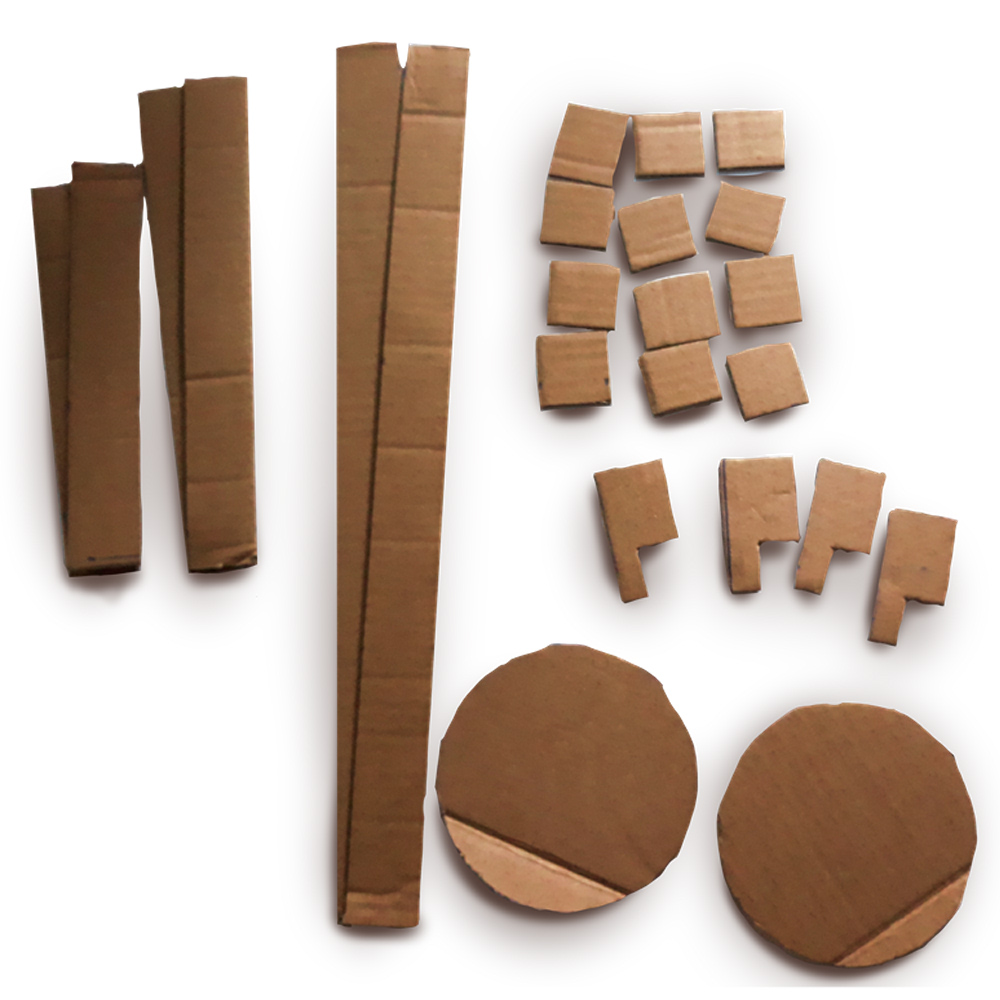
\includegraphics[width=5cm]{pappstucke.jpg}
\caption*{Stifte}
\end{figure}

}

\schritt{2}{Den Roboterarm bauen}{
Die Pappteile müssen zu einem Arm zusammengebaut werden. Dabei bilden zwei kleine Pappquadrae und ein Zahnstocher ein Gelenk, das die Pappteile miteinander verbindet.
Am besten orientiert ihr euch an der folgenden Grafik:\\

\begin{figure}[h]
\centering
\parbox{5cm}{
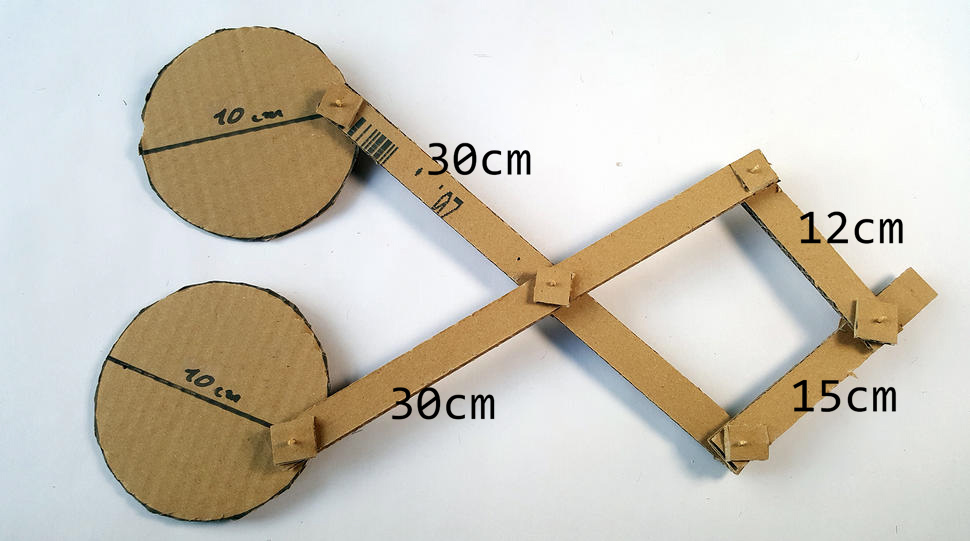
\includegraphics[width=5cm]{arm.jpg}
\caption*{Der fertige Roboterarm sollte sich leicht bewegen lassen.}
\end{figure}

Falls ihr nicht weiterwisst, gibt es auch eine ausführlichere Beschreibung auf https://tuduu.org/projekt/automatischer-malroboter .\\
Den Pappblock klebt ihr auf die Unterseite des Arms, also nicht die Fläche, auf welcher der zweite Pappstreifen aufliegt.\\

Wenn alles zusammengesteckt und verbunden ist, testet euren Arm vorsichtig. Bewegt sich alles reibungslos?\\
Dann verklebt die Zahnstocher zum Schluss oben und unten mit einem Tropfen Heißkleber, dann hällt alles ein bisschen besser.\\
Die Pappkreise klebt ihr so auf die Reifen, dass die Pappstreifen oben auf liegen.\\


%%%%%%%%%%%%%%%%%%%%%%%%%%%%%%





}


\subsection{Verbindung mit RaspberryPi}

\begin{center}
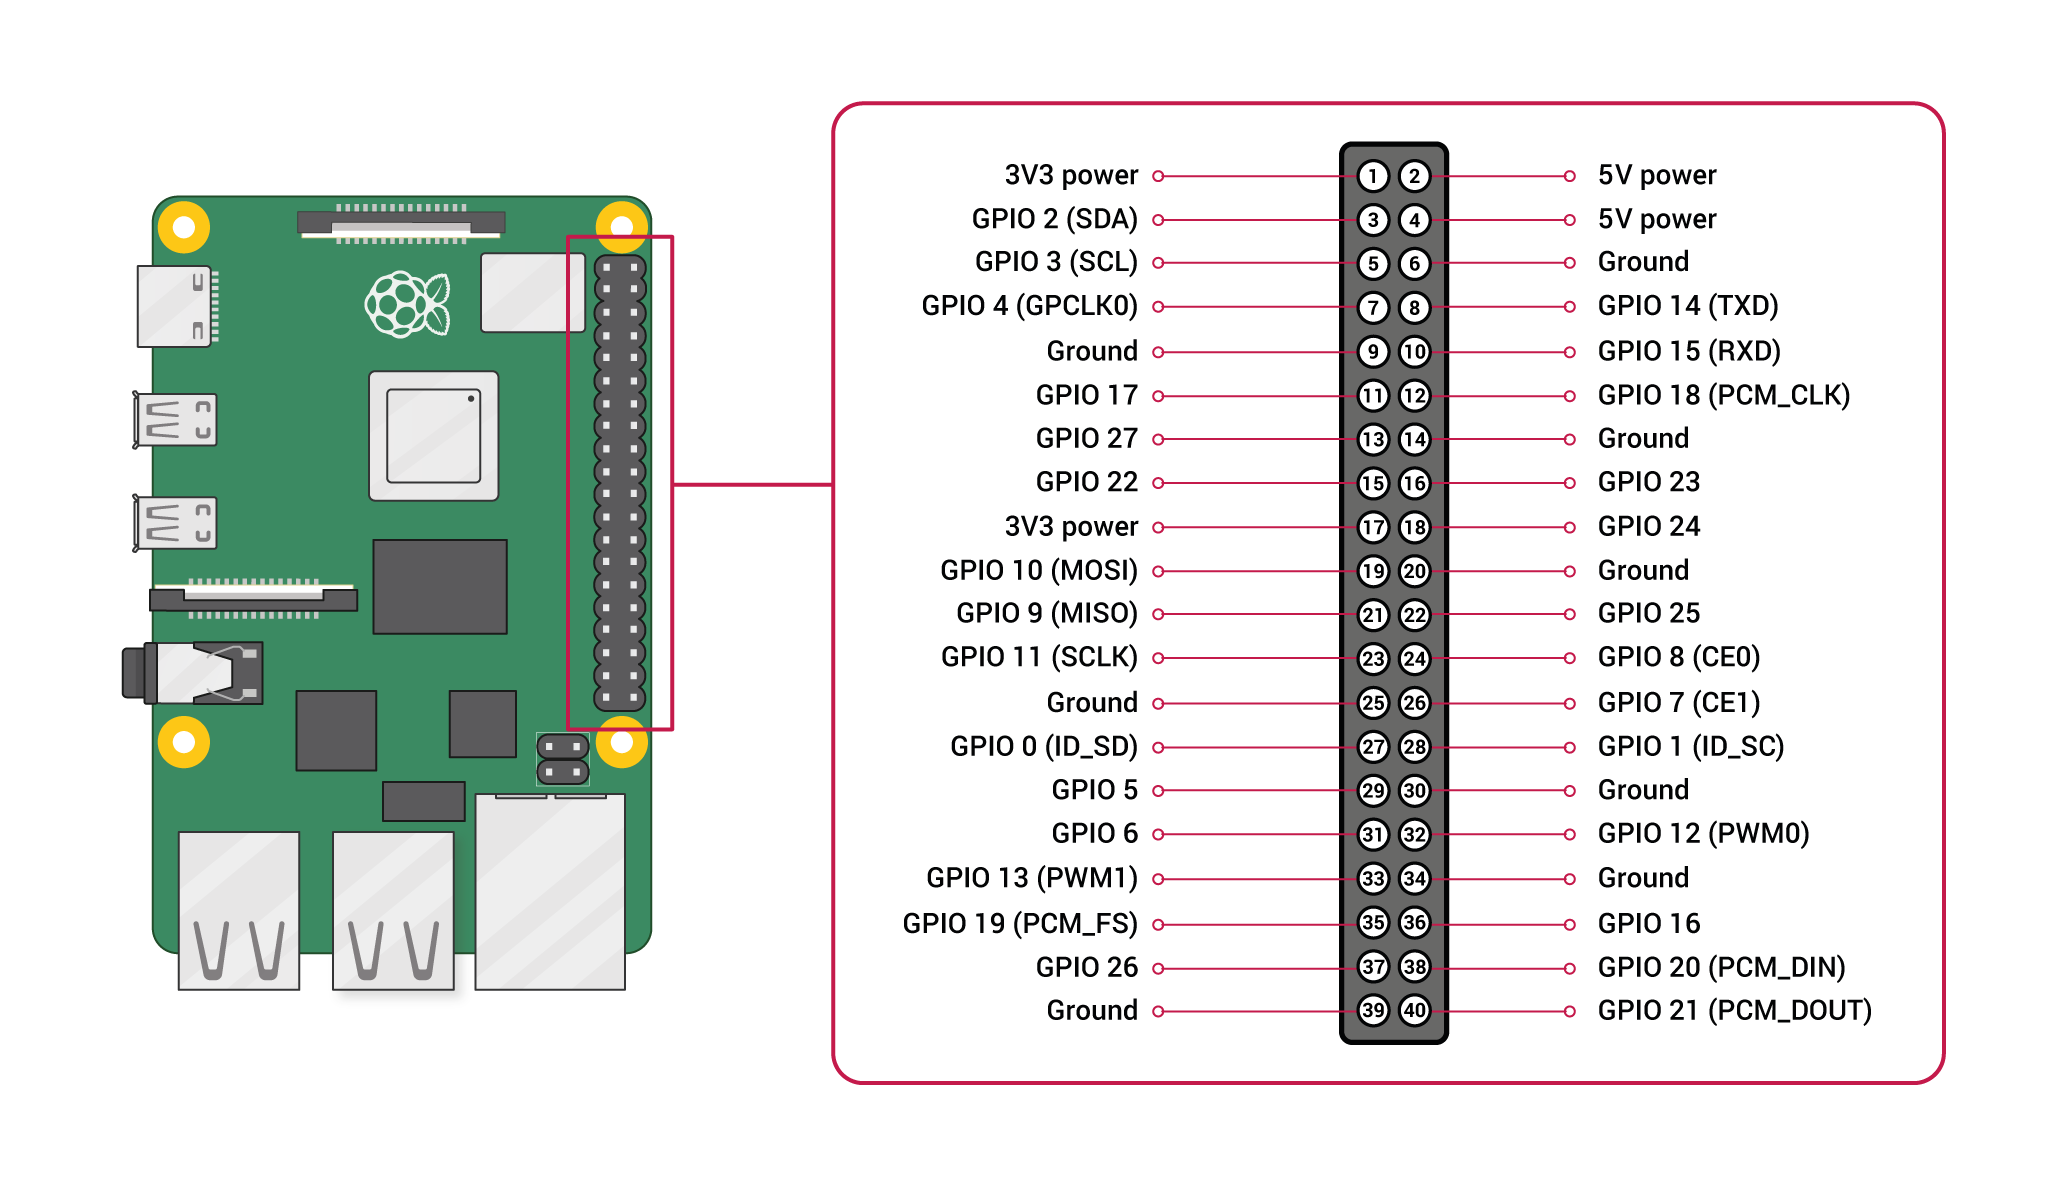
\includegraphics[width=\textwidth]{rpi_gpio_pinout.png}
\end{center}

\subsubsection{Verbindung Motor mit Treiber}
\subsubsection{Verbindung Treiber mit RaspberryPi}

\subsection{Programmierung}
\subsection{Programm A (Beispiel)}
\subsection{Programm B}
